\documentclass{article}

\usepackage[most]{tcolorbox}
\usepackage{physics}
\usepackage{graphicx}
\usepackage{float}
\usepackage{amsmath}
\usepackage{amssymb}


\usepackage[utf8]{inputenc}
\usepackage[a4paper, margin=1in]{geometry} % Controla los márgenes
\usepackage{titling}

\title{Clase 16}
\author{Manuel Garcia.}
\date{\today}

\renewcommand{\maketitlehooka}{%
  \centering
  \vspace*{0.05cm} % Espacio vertical antes del título
}

\renewcommand{\maketitlehookd}{%
  \vspace*{2cm} % Espacio vertical después de la fecha
}

\newcommand{\caja}[3]{%
  \begin{tcolorbox}[colback=#1!5!white,colframe=#1!25!black,title=#2]
    #3
  \end{tcolorbox}%
}

\begin{document}
\maketitle

\section{Derivada}
\textbf{Ejemplo: } Derivar $ f(z) = \bar z  $
\begin{gather*}
  f'(z) = \underset{\Delta z  \rightarrow 0 }{lim}\frac{f(z + \Delta z ) - f(z) }{\Delta z }\\
  \underset{\Delta z  \rightarrow 0 }{lim}\frac{\overline{z + \Delta z } - \bar z }{\Delta z } = \underset{\Delta z  \rightarrow 0 }{lim}\frac{\bar z + \overline{\Delta z} - \bar z }{\Delta z } = \underset{\Delta z  \rightarrow 0 }{lim}\frac{\bar{\Delta z }}{\Delta z }\\
  = \underset{\Delta x , \Delta y  \rightarrow 0,0 }{lim}\frac{\Delta x - i \Delta y }{\Delta x + i \Delta y } = \underset{\Delta y  \rightarrow 0 }{lim}\frac{-i  \Delta y }{i \Delta y  } = - 1\\
  \text{Por otro lado }\\
  \underset{\Delta y , \Delta x  \rightarrow 0,0 }{lim}\frac{\Delta x - i \Delta y }{\Delta x + i \Delta y } = \underset{\Delta x  \rightarrow 0 }{lim}\frac{\Delta x }{\Delta x } = 1 
\end{gather*}
Por ambos lados el limite es diferente por lo tanto no existe.

\textbf{Ejemplo: } Derivar $ f(z) = \left(2 z ^2 + 6 z + 5 \right)^3  $ evaluada en $ z = 1 + 2 i  $. Se puede utilizar la \textbf{derivada compuesta } $ (f \circ g )' = 3 (3z ^2 + 6 z + 5 ) ^2 (6z + 6 ) $
\begin{gather*}
  f'(z) = 3 (3 z ^2 + 6 z + 5 )^2 (6z + 6 ) = -17136i - 14048 
\end{gather*}

\section{Ecuaciones de Cauchy-Riemann }
Sea $ f(z) = u + i v  $, vamos a calcular el límite que define a la derivada por dos caminos especificos:
\begin{figure}[H]
  \begin{center}
    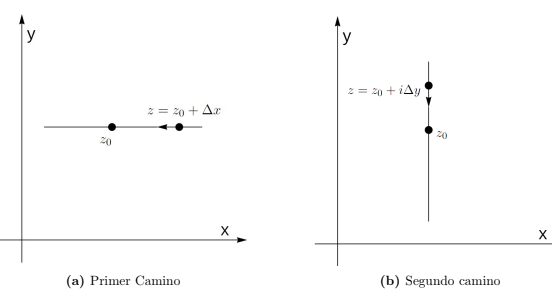
\includegraphics[width=0.6\textwidth]{cauchy-riemann.png}
  \end{center}
\end{figure}
\begin{align*}
  f'(z_0) &= \underset{\Delta x  \rightarrow 0 }{lim}\frac{f(x_0 + i y + \Delta x ) - f(x_0 + i y_0 )}{\Delta x }\\ 
          &= \underset{\Delta x  \rightarrow 0 }{lim}\frac{u(x_0 + \Delta x, y_0 ) + i v(x_0 + \Delta x , y_0 ) - u (x_0 , y_0 ) + i v (x_0,y_0 )}{\Delta x }\\
          &= \underset{\Delta x  \rightarrow 0 }{lim}\frac{u (x_0 + \Delta x , y_0 ) - u (x_0, y_0 )}{\Delta x } + i \underset{\Delta x  \rightarrow 0 }{lim}\frac{v(x_0 + \Delta x , y_0 ) - v (x_0,y_0 )}{\Delta x }\\
          &= \frac{\partial u  }{\partial x } + i \frac{\partial v  }{\partial x }
\end{align*}
Por el otro camino: 
\begin{align*}
  f'(z_0) &= \underset{\Delta y  \rightarrow 0 }{lim}\frac{f(z_0 + i y _0 + i \Delta y ) - f(x_0 + i y_0 )}{i \Delta y }\\
          &= \underset{\Delta y  \rightarrow 0 }{lim}\frac{u (x_0, y_0 + \Delta y ) - u (x_0,y_0 ) + i[v(x_0,y_0 + \Delta y ) - v (x_0,y_0 )]}{i \Delta y }\\
          &= -i \frac{\partial u  }{\partial y } + \frac{\partial v  }{\partial y }
\end{align*}
Necesitamos que la parte real de la ecuacion por el primer lado sea igual que en la del segundo lado, y lo mismo con la parte compleja. De esta forma obtenemos las ecuaciones de Cauchy-Riemann: 
\caja{red}{Ec. Cauchy-Riemann}{
\begin{itemize}
    \item $ \displaystyle{\frac{\partial u  }{\partial x } = \frac{\partial v  }{\partial y }} $
    \item $ \displaystyle{\frac{\partial v  }{\partial x } = - \frac{\partial u  }{\partial y }} $
  \end{itemize}
}
\textbf{Ejemplo: }derivar $ f(z) = (z ^2 + 5 i z + 8 ) ^2  $
\begin{align*}
  f(z) &= z ^4 - 25 z ^2 + 64 + 10iz^3 + 16 z ^2 + 80i z\\
       &= (x + i y)^4 - 25 (x + i y )^2 + 64 + 10i(x + i y )^2 + 80 i (x + i y)\\
       &= x ^4 + 4 x ^3 (iy) + 6 x^2 (iy)^2 + 4 x (iy)^3 + (iy)^4 - 9 (x^2 + 2 i xy + (iy)^2) + 64 + 10i (x^3 + 3x^2 (iy) + 3x (iy)^2\\ &+ (iy)^3) + 80i(x + iy)\\
       &= x^4 + 4i x^3 y - 6x^2y^2 - 4ixy^3 + y^4 - 9x^2 - 18 i xy + 9 y^2 + 64 + 10ix^3 - 30 x^2 y  - 30ixy^2 + 10 y^3 + 80ix - 80y
\end{align*}
Tenemos que: 
\begin{gather*}
  u(x,y) = x^4 - 6x^2y^2 + y^4 - 9x^2 + 9y^2 + 64 - 30x^2y + 10y^3 - 80y\\
  v(x,y) = 4x^3 y - 4 x y^3 - 18xy + 10x^3 - 30xy^2 + 80x
\end{gather*}
Haciendo las derivadas: 
\begin{gather*}
  \frac{\partial u  }{\partial x } = 4x^3 - 12 x y ^2 - 18 x - 60xy\\
  \frac{\partial v  }{\partial  x } = 12x^2y - 4 y ^3 - 18y + 30x^2 - 30y^2 + 80\\
  \frac{\partial u  }{\partial y } = - 12 x^2 y + 4 y^3 + 18 y - 30 x^2 + 30 y ^2 - 80 \\
  \frac{\partial v  }{\partial y } = 4x^3 - 12 x y^2 - 18 x - 60 xy 
\end{gather*}
Como cumple las ecuacion de cauchy-riemann no podemos decir que la derivada existe pero si no cumpliera las ec. entonces no existiria la derivada.

\textbf{Ejemplo: } Compobrar las ecuacion de Cauchy-Riemann para $ f(z) = i \bar z^2 + 2 \bar z  $.
\begin{align*}
  f(z) &= i \bar z ^2 + 2 \bar z \\ 
  &= i (x^2 - 2 xy i - y^2) + 2x - 2iy \\
  u (x,y) = 2xy + 2x \qquad \qquad v(x,y) = -2y + x^2 - y^2 \\
  \frac{\partial u  }{\partial x } = 2y + 2 \qquad \qquad \frac{\partial v  }{\partial x } = 2x \\
  \frac{\partial u  }{\partial y } = 2x \qquad \qquad \frac{\partial v  }{\partial y } = -2-2y
\end{align*}
No cumple las ecuaciones de Cauchy-Riemann.

\subsection{Cauchy-Riemann en polares }
\begin{gather*}
  \frac{\partial u  }{\partial x } =  \frac{\partial u  }{\partial  r } \frac{\partial r  }{\partial x } + \frac{\partial u  }{\partial \theta } \frac{\partial \theta  }{\partial x }\qquad \qquad
  \frac{\partial u  }{\partial y } = \frac{\partial u  }{\partial r } \frac{\partial r  }{\partial y } + \frac{\partial u  }{\partial \theta } \frac{\partial \theta  }{\partial y }\\
  \frac{\partial v  }{\partial  x } = \frac{\partial v  }{\partial r } \frac{\partial r  }{\partial x } + \frac{\partial v  }{\partial \theta }\frac{\partial \theta  }{\partial x }\qquad \qquad
  \frac{\partial v  }{\partial  y } = \frac{\partial v  }{\partial r }\frac{\partial r  }{\partial y}  + \frac{\partial v  }{\partial  \theta } \frac{\partial \theta  }{\partial  y }
\end{gather*}
Ademas podemos comprobar que: 
\begin{gather*}
  \frac{\partial r  }{\partial x } = \cos{\theta} \qquad \qquad \frac{\partial \theta  }{\partial x } = - \frac{\sin{\theta }}{r } \\
  \frac{\partial r  }{\partial y} = \sin{\theta} \qquad \qquad \frac{\partial \theta  }{\partial y} = \frac{\cos{\theta}}{r}
\end{gather*}
Reemplazando en las derivadas parciales de $ u  $ y de $ v  $: 
\begin{gather*}
  u_x = u_r \cos{\theta} - u _\theta \frac{ \sin{\theta} }{ r } \qquad \qquad u_y = u_r \sin{\theta} + u_\theta  \frac{\cos{\theta}}{r }\\
  v_x = v_r \cos{\theta} - v_\theta \frac{\sin{\theta}}{r } \qquad \qquad v_y = v_r \sin{\theta} + v_\theta \frac{\cos{\theta}}{r}
\end{gather*}
Reemplazando en las ec. de Cauchy-Riemann: 
\begin{gather*}
  v_r \cos{\theta} - v_\theta \frac{\sin{\theta }}{r } =  -u_r \sin{\theta} - u _\theta \frac{\cos{\theta}}{r} \qquad \qquad u_r \cos{\theta} - u_\theta \frac{\sin{\theta}}{r } = v_r \sin{\theta} + v_\theta \frac{\cos{\theta}}{r }\\
  \text{Multiplicando por }\cos{\theta}\qquad \qquad \qquad \qquad \text{Multiplicando por }\sin{\theta}\\
  v_r \cos^2 \theta - v_\theta \frac{\sin{\theta}\cos{\theta}}{r } = - u_r \sin{\theta} \cos{\theta} - u_\theta \frac{\cos^2 \theta }{r } \qquad \qquad 
  v_r \sin^2 {\theta} + v_\theta \frac{\sin{\theta}\cos{\theta}}{r } = u_r \cos{\theta} \sin{\theta} - u_\theta \frac{\sin^2{\theta }}{r }
\end{gather*}
Entonces: 
\begin{gather*}
  v_r = - \frac{u_\theta }{r } \qquad \qquad u_r = \frac{v_\theta }{r} 
\end{gather*}


\end{document}
